% !Mode:: "TeX:UTF-8"

\chapter{超像素分割}

\begin{figure*}[h]
\begin{center}
%\fbox{\rule{0pt}{2in} \rule{.9\linewidth}{0pt}}
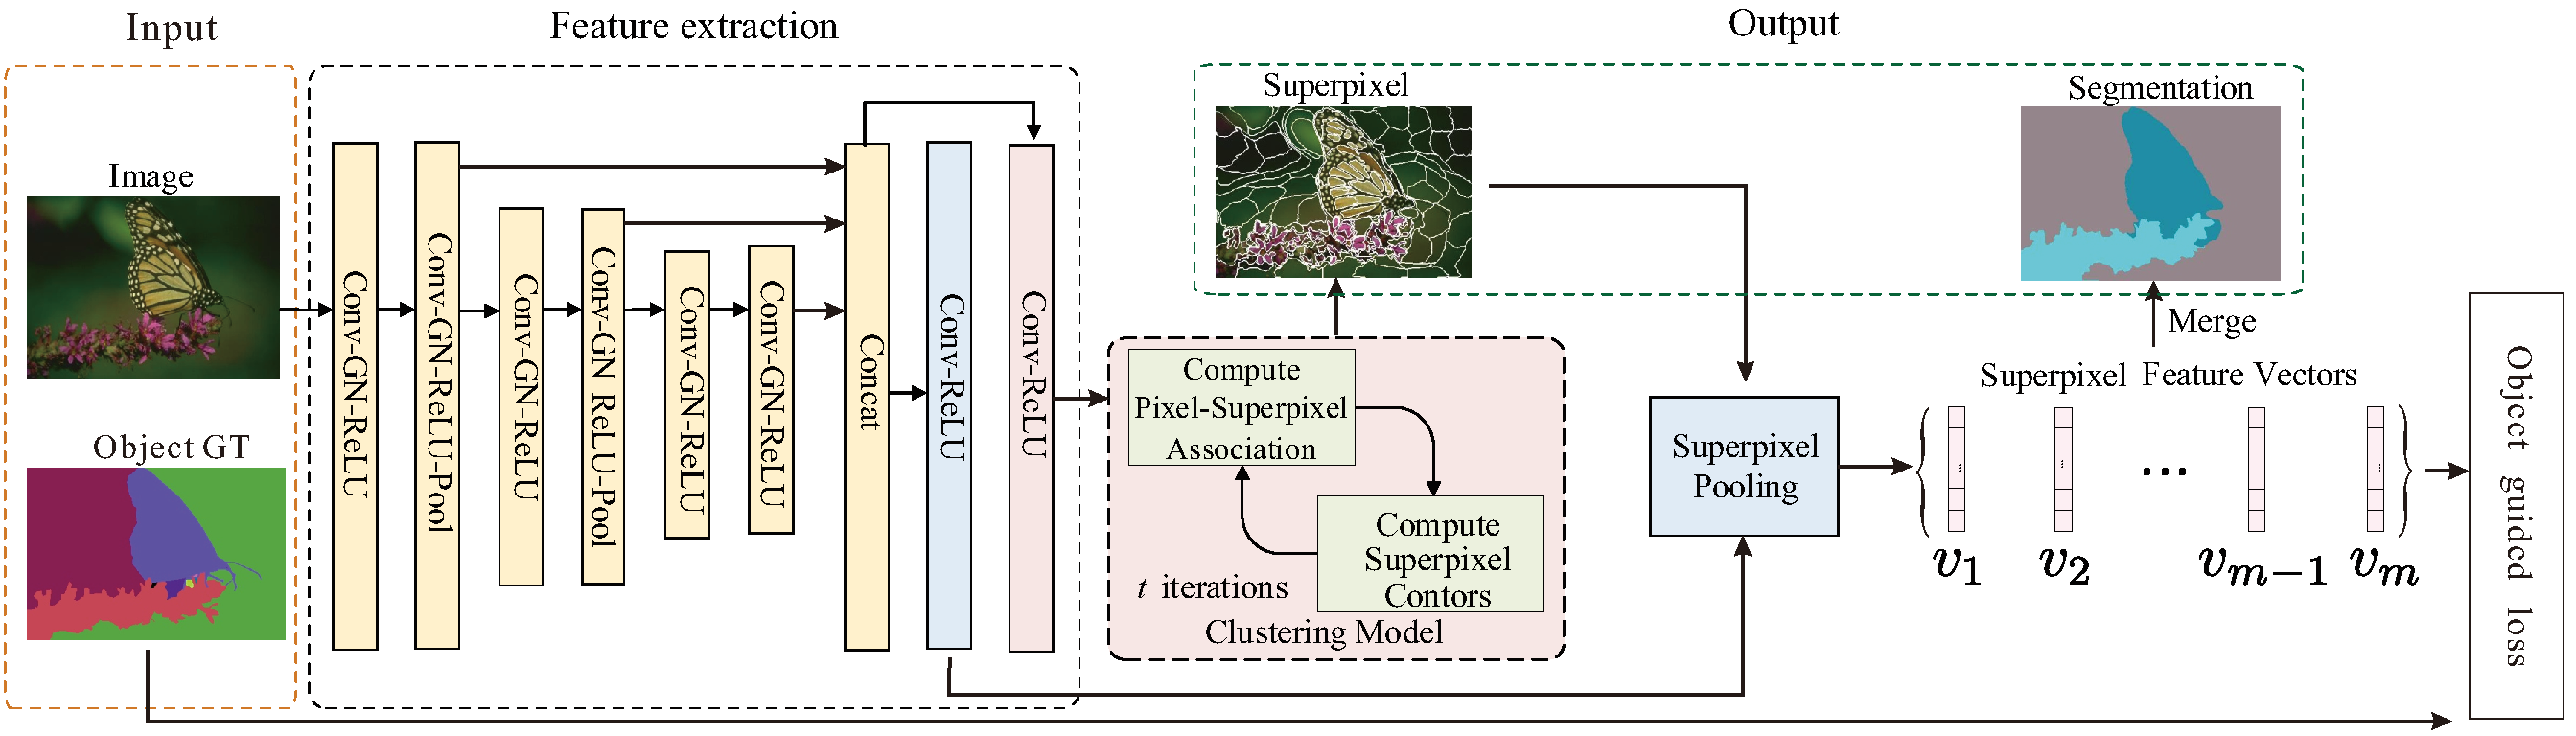
\includegraphics[width=1\textwidth]{figures/img/pipeline.pdf}
\end{center}
\vspace{-5mm}
\caption{算法流程图。对于给定的图像,我们的算法同时生成超像素和图像分割。输入图像首先被输送到一个特征提取网络,该网络由一系列卷积层、归一化(GN)和ReLU操作组成。然后将提取的特征输入可微聚类模块,生成超像素。超像素池用于获取超像素特征向量。最后通过合并相似度高的超像素实现图像分割}
\label{Fig.sub.1}
\end{figure*}

如图3-1所示,我们的方法首先从CNN深度网络中学习图像特征,然后我们使用迭代可微分聚类算法模块来获取超像素。接下来,我们通过超像素池化层计算超像素特征向量,并计算相邻超像素之间的相似性。最后,根据相似度判断相邻的两个超像素是否合并。在本节中,我们将详细介绍我们的方法。

\section{超像素生成}

超像素将相似像素分组为各向同性区域,从而可以提高分割质量和效率。 例如,在DEL算法中,作者使用SLIC作为图像分割的开始。在本文中,与采用现有的超像素算法进行图像分割的方法不同,我们将超像素生成作为图像分割网络的一部分。为此,我们采用SSN中提出的可微聚类算法模块,以取代SLIC算法中的硬像素-超像素关联。

通常,对于$n$像素的图像\(I\in\mathbb{R}^{n\times 5}\),在CIELAB空间的特征为$I_p=[x,y,l,a,b]$ ,我们希望将其划分为$m$ 个小区域,即将图片分成m个超像素。在介绍在描述软关联之前,我们简要介绍SLIC算法中如何计算像素-超像素硬关联$H = \left \{1, 2, \cdots, m \right \}^{n\times 1}$。给定统一采样的超像素中心$C^{0}$作为初始值,SLIC算法在每次迭代$t$中计算每个像素$p$处的新超像素分配,
\begin{equation}\label{eqn:hardassn}
H_{p}^{t} =  \mathop{{{\rm argmin}}}\limits_{{i\in\{ 1, 2, \cdots ,m \} }}\left\|I_{p}-C_{i}^{t-1}\right\|_2,
\end{equation}
其中$\|\cdot\|_2$表示输入向量的$\ell_2$范数,$C_i^{t-1}$表示超像素中心$i$的特征,该特征通过对第$t$次迭代后,计算属于该超像素中心的像素的特征平均值来获取。

由于(3-1)获取像素-超像素硬关联H的操作是不可微的,因此SLIC无法直接集成到神经网络中。 在我们算法中的用到的可微分聚类算法模块,其将硬像素-超像素硬关联H替换为软关联Q。与原始SLIC相似,它在每次迭代中具有以下两个核心步骤:

1.	像素-超像素关联计算。第t次迭代中像素p及其相邻超像素i之间的关联计算如下:
\begin{equation}
Q_{pi}^{t} = e^{-\left \| F_{p}-C_{i}^{t-1}\right \|_2^2},
\end{equation}
其中\(F_{p}\)是像素$p$的深层特征。 在我们的情况下,它来自我们网络的特征提取模块。\(Q_{pi}^{t}\)是$t$次迭代后像素$p$与超像素中心$i$之间的距离。

2.	超像素中心更新。新的超像素聚类中心是根据像素特征的加权总和得出的,
\begin{equation}
C_{i}^{t} = \frac{1}{Z_{i}^{t}}\sum_{p}Q_{pi}^{t}F_{p},
\end{equation}
其中$Z_{i}^{t}$表示归一化过程,即$Z_{i}^{t} = \sum\nolimits_{p}Q_{pi}^{t} $ 。

将这两个步骤迭代数次(在本文中,设定迭代次数为10次),最终得到像素-超像素软关联\(Q\in\mathbb{R}^{n\times m}\)。与(3-1)相似,我们需要计算硬关联映射$H'\in \mathbb{R}^{n\times 1}$,最终得到像素$p$的超像素标签,
\begin{equation}
H'_{p} =  \mathop{{{\rm argmax}}}\limits_{{i \in \left\{ 1, \cdots ,m \right\} }}Q_{pi}.
\label{equation.3}
\end{equation}

值得注意的是,这种硬关联的计算是不可微的。因此在我们的算法中,这一步不参与反向传播。在实验中,我们发现计算像素和超像素聚类中心之间的软关联非常耗时。与SLIC相似,我们只是计算每个像素到周围超像素聚类中心的距离,大大减少了计算时间。

